Artificial Intelligence (A.I.) systems are becoming increasingly prevalent in
modern consumer products.  Google's ``Google Now" system determines
what information its user wants to see before they ask for it.  Apple's ``Siri"
acts as an artificial personal assistant, attempting to respond to queries stated in
natural language.  Android (which includes Google Now) and iOS (which
includes Siri) have 45\% market penetration between them, and there were
470 million smartphones sold in 2011, with expectations of increase in 2012 and 2013
 \cite{smartphones}.

Visions of future A.I. systems have long included natural
language interfaces.  The ship's computer from Star Trek, the robots from
the works of Heinlein and Asimov, and the droids from Star Wars are
all capable of human speech, and even those which are not capable of dialogue
are able to receive orders verbally and respond in kind.  A system 
for understanding and creating language is a fundamental part of
an artificial intelligence like humans have been imagining for many years.

Consequently, a crucial subcomponent of artificial intelligence is Natural Language Processing (NLP).
NLP studies the task of interacting with humans using languages which are inherently
complex and ambiguous (e.g. English).
In order to successfully communicate with people, a system which does natural
language processing will need to accept language as input
and translate it into a format that computers can work with.  Such a system will also
need to be able to translate from an internal meaning representation to natural language.
See Figure \ref{nlp-block} for a visual explanation of this process.

For example, consider a robotic concierge system which takes phone calls from users.
A system like this has been shown to be practical \cite{litman_njfun_2000}, so it serves
as a good example of an interaction with a system capable of generating language.
One possible interaction might be the following:

\begin{verbatim}
Computer:  How may I help you today?
User    :  I am looking for a place to eat dinner.
\end{verbatim}

Once the user has finished speaking, the computer system has a series of electrical signals on
a phone line which it will need to decode into human speech.  This is the first step
in the block diagram of Figure \ref{nlp-block}.  Let us assume that this step proceeds without
error.  At this point, the computer system will need to attempt to understand the natural
language input of ``I am looking for a place to eat dinner". One very simple possibility is
a straightforward keyword-searching approach.  Such an approach might look for the words ``I",
``place", ``eat", and ``dinner", and determine that the speaker desires a listing of restaurants that
are open for dinner.  This is the ``NLP Parsing" step of Figure \ref{nlp-block}.  The system would
then do some internal processing (e.g. database queries), which makes up the ``Processing"
step.  The system may determine that it needs to respond to the user, perhaps to ask a
clarifying question to narrow the user's search.  This determination will be made in the
``Response Generation" block.  At this point, the system will have an internal representation
of the type of question it needs to ask which we call a ``communicative goal".  That goal might
look something like the following:
\begin{verbatim}
question type: clarifying
question seeks: preferences
question regards: dinner type
question language: English
\end{verbatim}

The computer system next needs to translate that into a sentence in its output
language.  The process of going from this internal representation to text like
``What type of food do you typically enjoy for dinner?" is called Natural Language Generation,
and comprises the fifth block of the NLP process.  Finally, this generated text is conveyed to
the user by encoding it into the data that can travel over a telephone, using a text-to-speech
program.

As this example shows, even without the aforementioned lofty future goals,
the increasing frequency of natural language interfaces for consumer
products shows that natural language generation (NLG) is becoming more and more important
in the world.  Consequently, a consistent and reliable method for creating a natural
language generation system would be of value, especially if the system's
computational requirements were small enough that the system could be embedded
in consumer electronics.

\begin{figure}
\centering
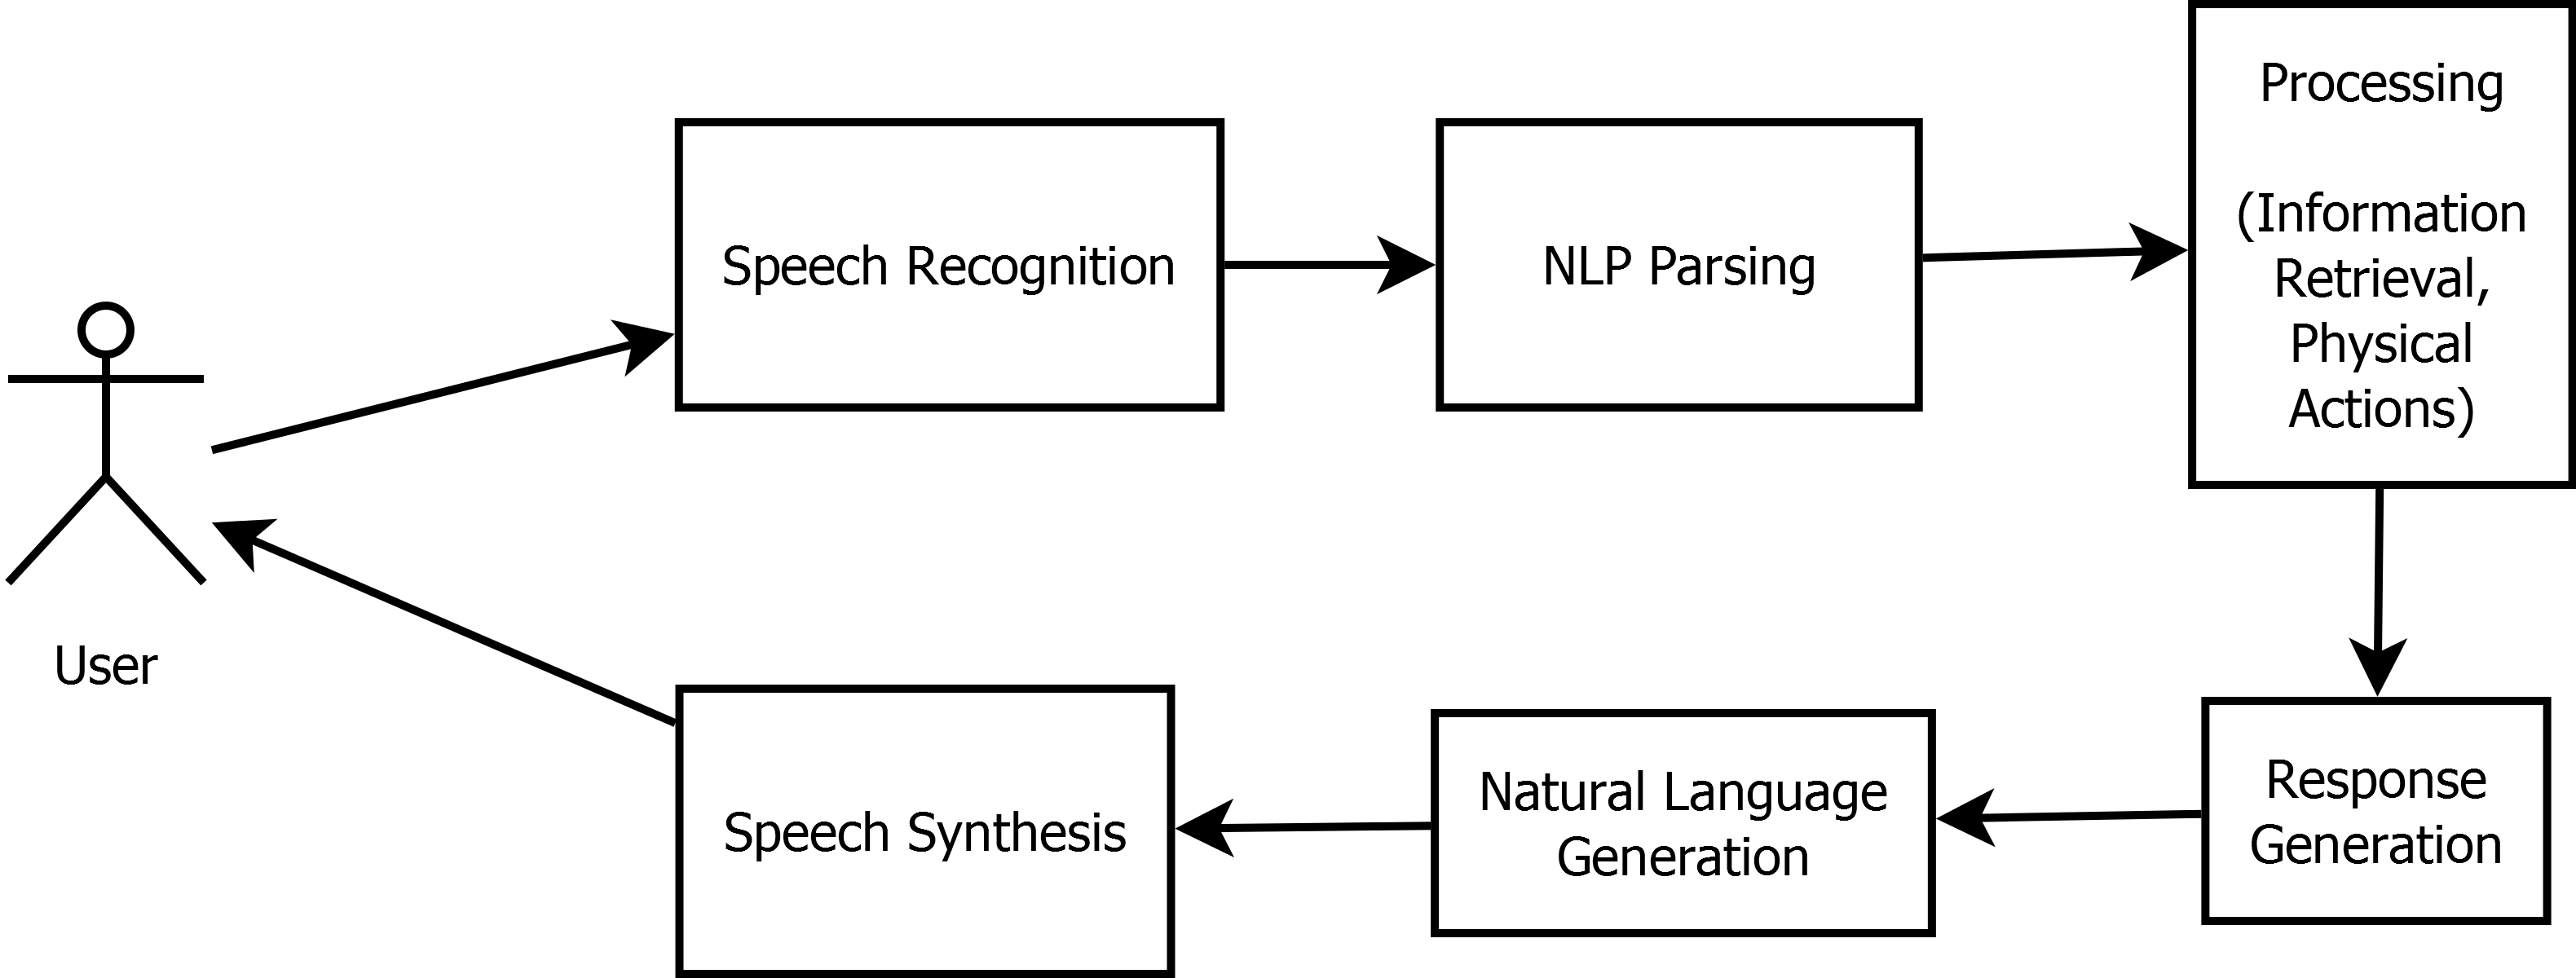
\includegraphics[width=0.8 \linewidth]{nlp-block.png}
\caption{The flow of information through a normal interaction
with a user in a generalized NLP system}
\label{nlp-block}
\end{figure}

In this thesis, we consider the following restricted NLG problem: given a
grammar, lexicon, and a communicative goal, output a valid English
sentence that satisfies this goal.  We call this problem "restricted", because
it assumes a level of knowledge about the context in which the generation
will occur.  In principle, the most general NLG problem is to produce a valid
sentence in an arbitrary language, using the entire grammar and lexicon available
in that language, to satisfy an arbitrary communicative goal.  In practice, we
rarely require this level of generality; for instance, it would be unnecessary for the concierge
program described above to be intimately familiar with highly technical jargon.
We therefore start with this restricted subproblem, and plan to extend it in future work.

Previous work on this problem has taken two broad approaches.  On one hand we have
the classical planning approaches, which treat the problem of NLG as an AI planning
problem.  These systems have the advantage of being capable of finding acceptable
output in all circumstances where a perfect answer exists, but the disadvantage of
being unable to handle a probabilistic grammar in a structured way.  They also struggle
with completing a subset of the communicative goals, when full completion is not
possible.  On the other hand, there are statistical techniques which are not goal-directed.
These techniques work by examining the
most probable combinations of words and determining if any of those match the
meaning they are attempting to generate.  These have the advantage of completing
execution very quickly, and of taking advantage of Zipf's Law, which states broadly that
a very small subset of a language is used a very large proportion of the time.  They
have the disadvantage of requiring an inordinate amount of memory to be able to search
for the less-likely phrases and sentences which will occasionally need to be generated.
They also scale poorly with large grammar sizes.

We propose an algorithm which unifies these two approaches, and has, to some extent,
the advantages of both.  This algorithm gives
us the ability to efficiently search a large space (all possible natural language outputs) for 
one of many valid outputs.  We support probability in a structured way and allow
for generation using a large grammar.  We support partial completion of the communicative
goal, but strive for full completion when it is possible.  We allow for generation to stop
at any time and will return a partially-complete result very quickly.

We do this, broadly, by using probabilistic planning rather than classical planning.
Our algorithm is based on Monte-Carlo Tree Search \cite{kocsis_bandit_2006}, an increasingly
popular method for probabilistic planning.  This algorithm performs ``simulations",
examining different paths that generation could take and iteratively refining
the search based on how ``good" the outcomes of previous simulations were.
This ``goodness" is measured by a reward function which returns a numerical
estimation of the value of the generation.

We believe that if this algorithm were developed further, it could be useful as the
final step of a dialog system, or useful in generation situations where flexibility of the
generation system is crucial.  At present, it is already useful as the output stage of
a simple dialog system.  An efficient implementation would be able to take advantage
of multiprocessing and therefore run very well on a massively multiprocessing system,
enhancing performance substantially.

In chapter 2, we provide background information on NLG and probabilistic planning.  In chapter 3,
we discuss related work, including historical natural language generation frameworks.  We also
discuss the closest related system to ours, called CRISP.  In chapter 4, we present our framework
for natural language generation.  In chapter 5, we present our experimental evaluation of
our implementation, which shows that it performs comparably to the current state-of-the-art in
the field.  In chapter 6, we conclude by describing the potential applications and future work
using this method of generation.